\subsection{Residual Stream Basis}
\label{appendix:residual_stream_basis}

Figure \ref{fig:neuron_basis_apostrophe} gives a token activation histogram of the residual stream basis. Connecting this residual stream dimension to the apostrophe feature from Figure \ref{fig:apostrophe}, this residual dimension was the 10th highest dimension read from the residual stream by our feature\footnote{The first 9 did not have apostrophes in their top-activations like dimension 21.}. 

\begin{figure}[ht]
    \centering
    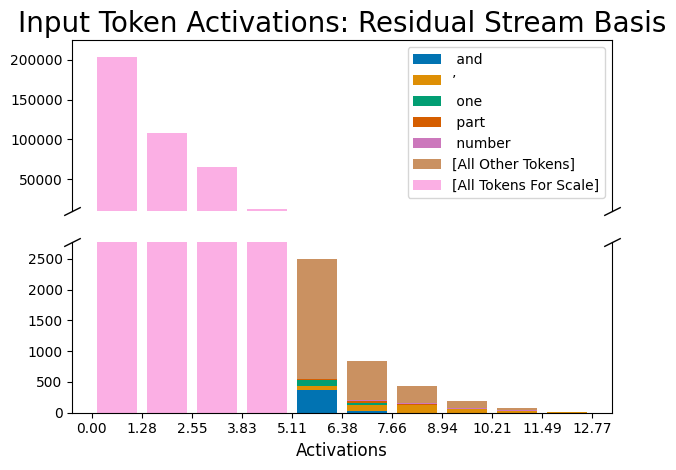
\includegraphics[width=0.8\textwidth]{images/logan/neuron_basis_21.png}
    \caption{Histogram of token counts in the neuron basis. Although there are a large fraction of apostrophes in the upper activation range, this only explains a very small fraction of the variance for middle-to-lower activation ranges.}
    \label{fig:neuron_basis_apostrophe}
\end{figure}


\subsection{Examples of Learned Features}
\label{appendix:learned_features_examples}


Other features are shown in Figures \ref{fig:if_feature}, \ref{fig:dis_feature}, \ref{fig:ill_feature}, and \ref{fig:dont_feature}.
\begin{figure}[ht]
    \centering
    \begin{minipage}[b]{0.45\textwidth}
        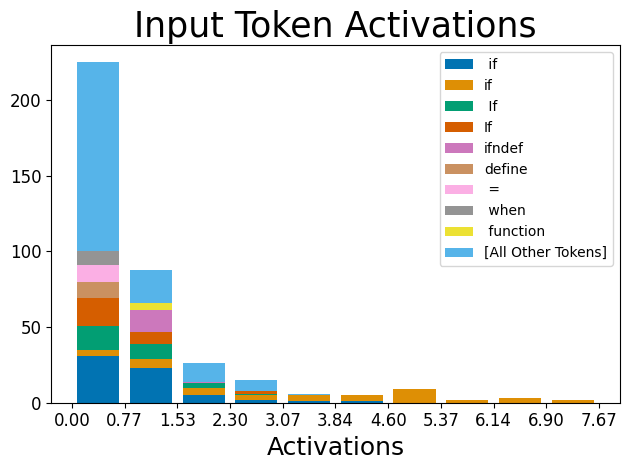
\includegraphics[width=\textwidth]{images/logan/if_feature.png}
    \end{minipage}
    \hfill  % Optional: To make sure they are as far apart as possible.
    \begin{minipage}[b]{0.45\textwidth}
        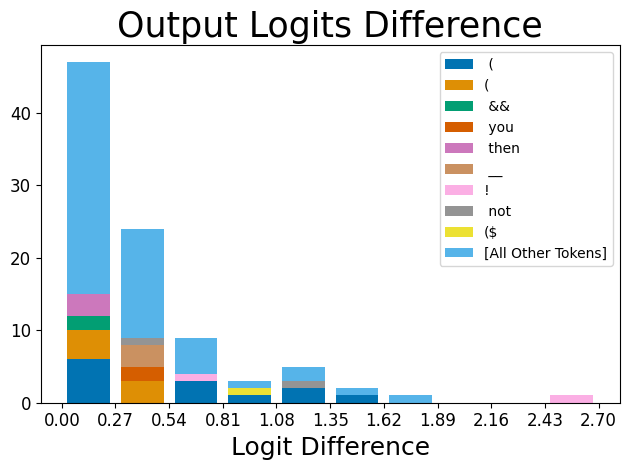
\includegraphics[width=\textwidth]{images/logan/if_feature_effect.png}
    \end{minipage}
    \caption{`If' feature in coding contexts}
    \label{fig:if_feature}
\end{figure}

\begin{figure}[ht]
    \centering
    \begin{minipage}[b]{0.49\textwidth}
        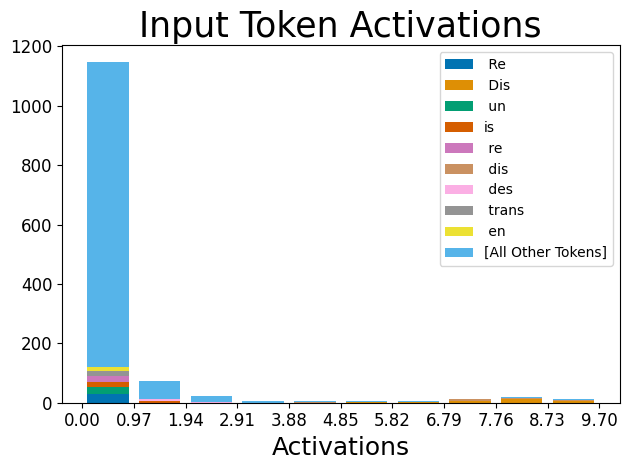
\includegraphics[width=0.9\textwidth]{images/logan/dis_feature.png}
    \end{minipage}
    \hfill  % Optional: To make sure they are as far apart as possible.
    \begin{minipage}[b]{0.49\textwidth}
        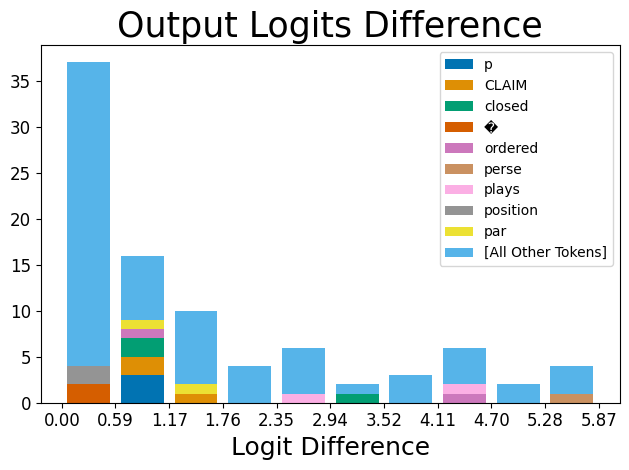
\includegraphics[width=0.9\textwidth]{images/logan/dis_feature_effect.png}
    \end{minipage}
    \caption{`Dis' token-level feature showing bigrams, such as `disCLAIM', `disclosed', `disordered', etc.}
    \label{fig:dis_feature}    
\end{figure}

\begin{figure}[ht]
    \centering
    \begin{minipage}[b]{0.49\textwidth}
        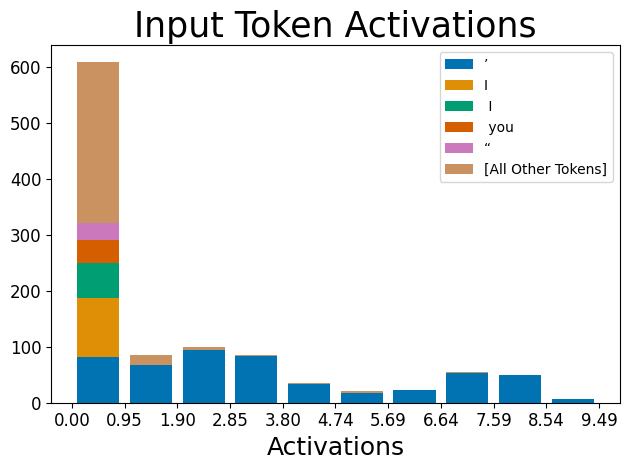
\includegraphics[width=0.9\textwidth]{images/logan/Ill_feature.png}
    \end{minipage}
    \hfill  % Optional: To make sure they are as far apart as possible.
    \begin{minipage}[b]{0.49\textwidth}
        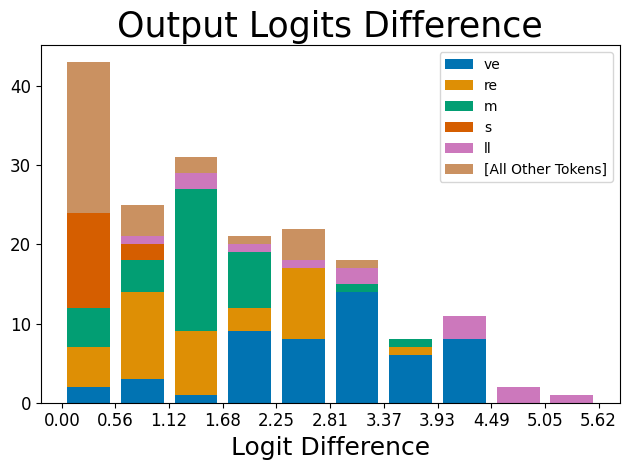
\includegraphics[width=0.9\textwidth]{images/logan/Ill_feature_effect.png}
    \end{minipage}
    \caption{Apostrophe feature in ``I'll"-like contexts.}
    \label{fig:ill_feature}
\end{figure}

\begin{figure}[ht]
    \centering
    \begin{minipage}[b]{0.49\textwidth}
        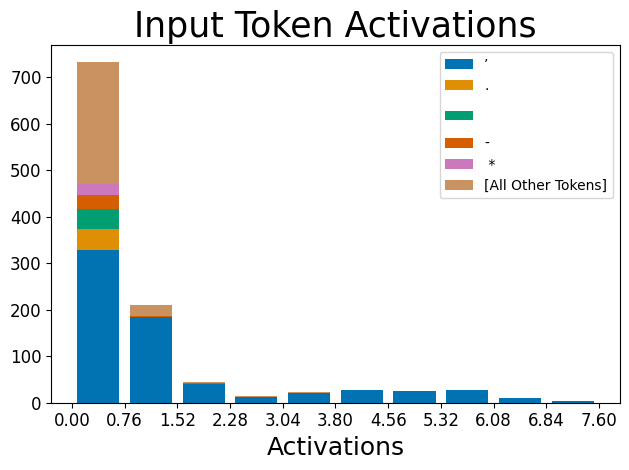
\includegraphics[width=0.9\textwidth]{images/logan/dont_feature.png}
    \end{minipage}
    \hfill  % Optional: To make sure they are as far apart as possible.
    \begin{minipage}[b]{0.49\textwidth}
        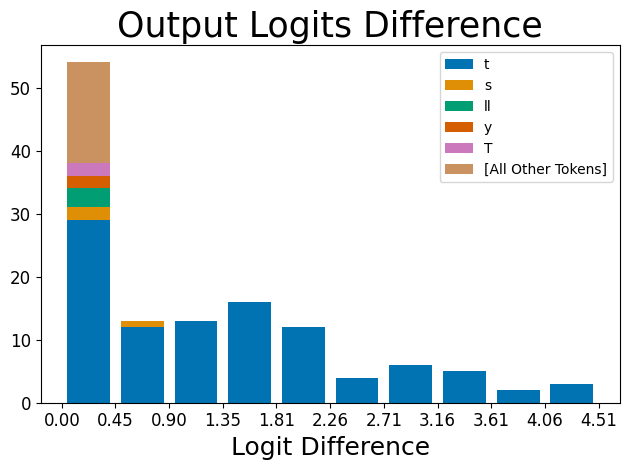
\includegraphics[width=0.9\textwidth]{images/logan/dont_feature_effect.png}
    \end{minipage}
    \caption{Apostrophe feature in ``don't"-like contexts.}
    \label{fig:dont_feature}
\end{figure}

% \begin{figure}
%     \centering
%     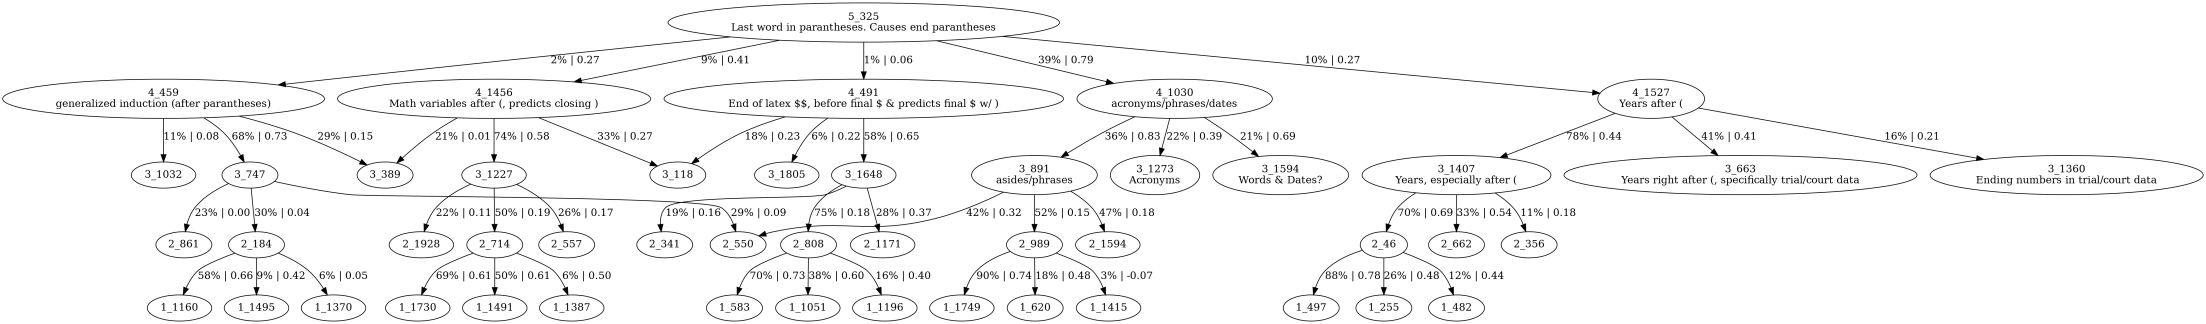
\includegraphics[width=0.9\textwidth]{images/network_place.png}
%     \caption{Closing parentheses graph. Percentage is the decrease in max-activating examples. Arrows are swapped. The other number is the cosine similarity between the two features.}
%     \label{fig:network_place}
% \end{figure}

\subsection{Feature Search Details}
\label{appendix:feature_search_details}

We searched for the apostrophe feature using the sentence `` I don't know about that. It is now up to Dave''', and seeing which feature (or residual stream dimension) activates the most for the last apostrophe token. The top activating feature in our dictionary was an outlier dimension feature (i.e., a feature direction that mainly reads from an outlier dimension of the residual stream), the apostrophes after O (and predicted O'Brien, O'Donnell, O'Connor, O'clock, etc), then the apostrophe-preceding-s feature. 

For the residual basis dimension, we searched for max and min activating dimensions (since the residual stream can be both positive and negative), where the top two most positive dimensions were outlier dimensions, the top two negative dimensions were our displayed one and another outlier dimension, respectively.

\subsection{Failed Interpretability Methods}
\label{appendix:failed_interp_methods}

We attempted a weight-based method going from the dictionary in layer 4 to the dictionary in layer 5 by multiplying a feature by the MLP and checking the cosine similarity with features in layer 5. There were no meaningful connections. Additionally, it's unclear how to apply this to the Attention sublayer since we'd need to see which position dimension the feature is in. We expected this failed by going out of distribution.
